The systematic uncertainty in the signal efficiency is estimated by estimating the systematic uncertainty of each efficiency factor in Eq.~\ref{eq:OverallEff}.

The systematic uncertainties on $\varepsilon_{\mathrm{track}}$, $\varepsilon_{\mathrm{vertexTrack}}$, and $\varepsilon_{\mathrm{vertexFit}}$ are studied using $K_{S}$ in Section~\ref{sec:syst_vertexing}. The systematic uncertainties on $\varepsilon_{\mathrm{lepton}}$ is studied in Section~\ref{sec:syst_leptonID} using tag-and-probe method with $Z\rightarrow ee,\mu\mu$ events. The systematic uncertainties on $\varepsilon_{\mathrm{trigger}}$ and $\varepsilon_{\mathrm{filter}}$ will be studied separately.

\subsection{Systematic uncertainties on tracking and vertexing efficiency}
\label{sec:syst_vertexing}
\subsubsection{Data and MC comparison}
\label{sec:vertexing_systematics_data_MC}
The systematic uncertainties on $\varepsilon_{\mathrm{track}}$, $\varepsilon_{\mathrm{vertexTrack}}$, and $\varepsilon_{\mathrm{vertexFit}}$ are estimated by comparing the tracking and vertexing efficiencies between the data and the background MC samples described in Section~\ref{sec:data_sample} using the process, $K_{S}\rightarrow\pi^{+}\pi^{-}$. In order to understand the validity and the limitation of this method, the kinematic distributions of $K_{S}$ and $Z'$ found in this method are compared in Appendix~\ref{app:syst_Ks_Zp}.

%In order to estimate the systematic uncertainties in reconstructing a displaced vertex, the tracking and vertexing efficiencies are compared between the data and the background MC samples described in Section~\ref{sec:data_sample} using $K_{S}\rightarrow\pi^{+}\pi^{-}$. % and its long lifetime ($c\tau \approx 26.84$ mm).

%The $K_{S}$ efficiency can be written as Eq.~\ref{eq:KaonEff}
%\begin{equation}
%\label{eq:KaonEff}
%\varepsilon_{K_{S}}=(\varepsilon_{\mathrm{track}}\cdot\varepsilon_{\mathrm{vertexTrack}})^2\cdot\varepsilon_{\mathrm{vertexFit}}=\bigg(\frac{N_{\mathrm{track}}}{N_{K_{S}}}\cdot\frac{N_{\mathrm{vertexTrack}}}{N_{\mathrm{track}}}\bigg)^2\cdot\frac{N_{\mathrm{vertex}}}{N_{\mathrm{trackPair}}}
%\end{equation}

Events are selected using the same event selection described in Section~\ref{sec:signal_selection}. %except trigger filter as electron or muon triggers are not useful for $K_{S}$ study. %In data sample, trigger applied?
From the selected events, $K_{S}$ candidates, referred as $K_{S}$ vertices, are selected by applying $K_{S}$ vertex selection to the secondary vertices in the events. $K_{S}$ vertex selection is similar to the $Z'$ signal vertex selection, but for the consistency with $K_{S}$ study in Run I and further background reduction, additional vertex cuts as described in Ref.~\cite{Aad:2011hd} are applied in $K_{S}$ vertex selection. The mass window of 0.35 to 0.65 GeV is used in the $K_{S}$ vertex selection. The difference between $K_{S}$ and $Z'$ vertex selections are summarized in Table~\ref{table:ks_vertex_cut}. Figure~\ref{fig:Ks_vertex_cutflow} shows $K_{S}$ vertex cut flow in the data and the background MC samples.

\begin{table}[!htb]
%\begin{table}[tb]
  \centering
  \begin{tabular}{ c c c }
    \hline
    \hline
    & $Z'$& $K_{S}$ \\
    \hline
    Vertex type & $\mu\mu$, $e\mu$, $ee$ & xx \\
    Mass (GeV) & $> 10.0$ & $[0.35,0.65]$ \\
    Additional cut & - & $K_{S}$ selection~\cite{Aad:2011hd} \\
    \hline
    \hline
  \end{tabular}
  \caption{Comparison of $Z'$ and $K_{S}$ vertex selections.}
  \label{table:ks_vertex_cut}
\end{table}

%\begin{figure}[tb]
\begin{figure}[!htb]
	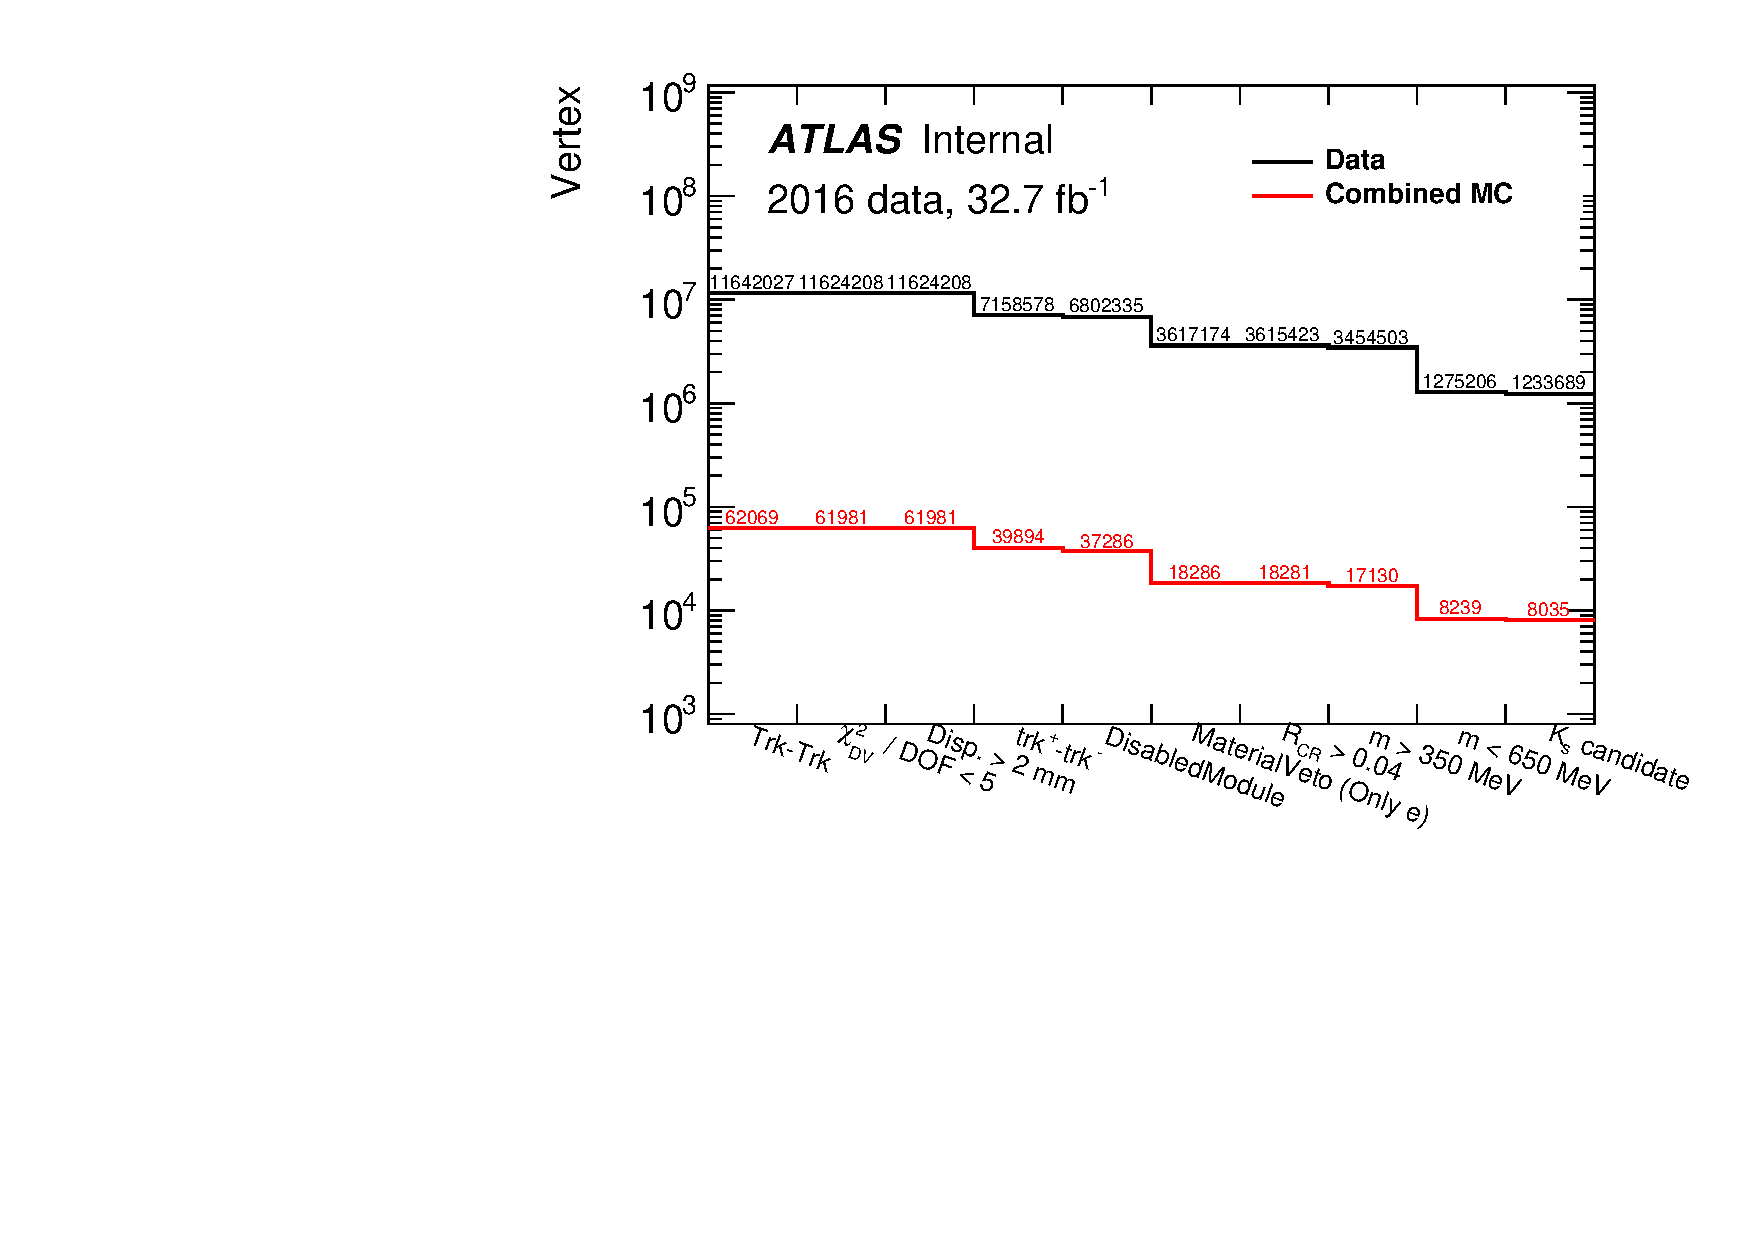
\includegraphics[width=0.60\textwidth]{figures/m_syst_Ks_cf.pdf}
	\centering
	\caption{Vertex cut flow applied on $K_{S}$ vertices in the data and MC samples}
	\label{fig:Ks_vertex_cutflow}
\end{figure}

After applying the event and $K_{S}$ vertex selection, the $K_{S}$ vertex distributions in the data are compared to the MC samples in Figure~\ref{fig:Ks_data_MC}. The data sample is normalized to the MC sample which has limited statistics. There are good agreements in the invariant mass, $p_{T}$, transverse, longitudinal position, and decay length of the vertices, except the pile-up distribution as expected.


\begin{figure}[!htb]
    \centering
    \subfloat[]{\label{subfig:Ks_m}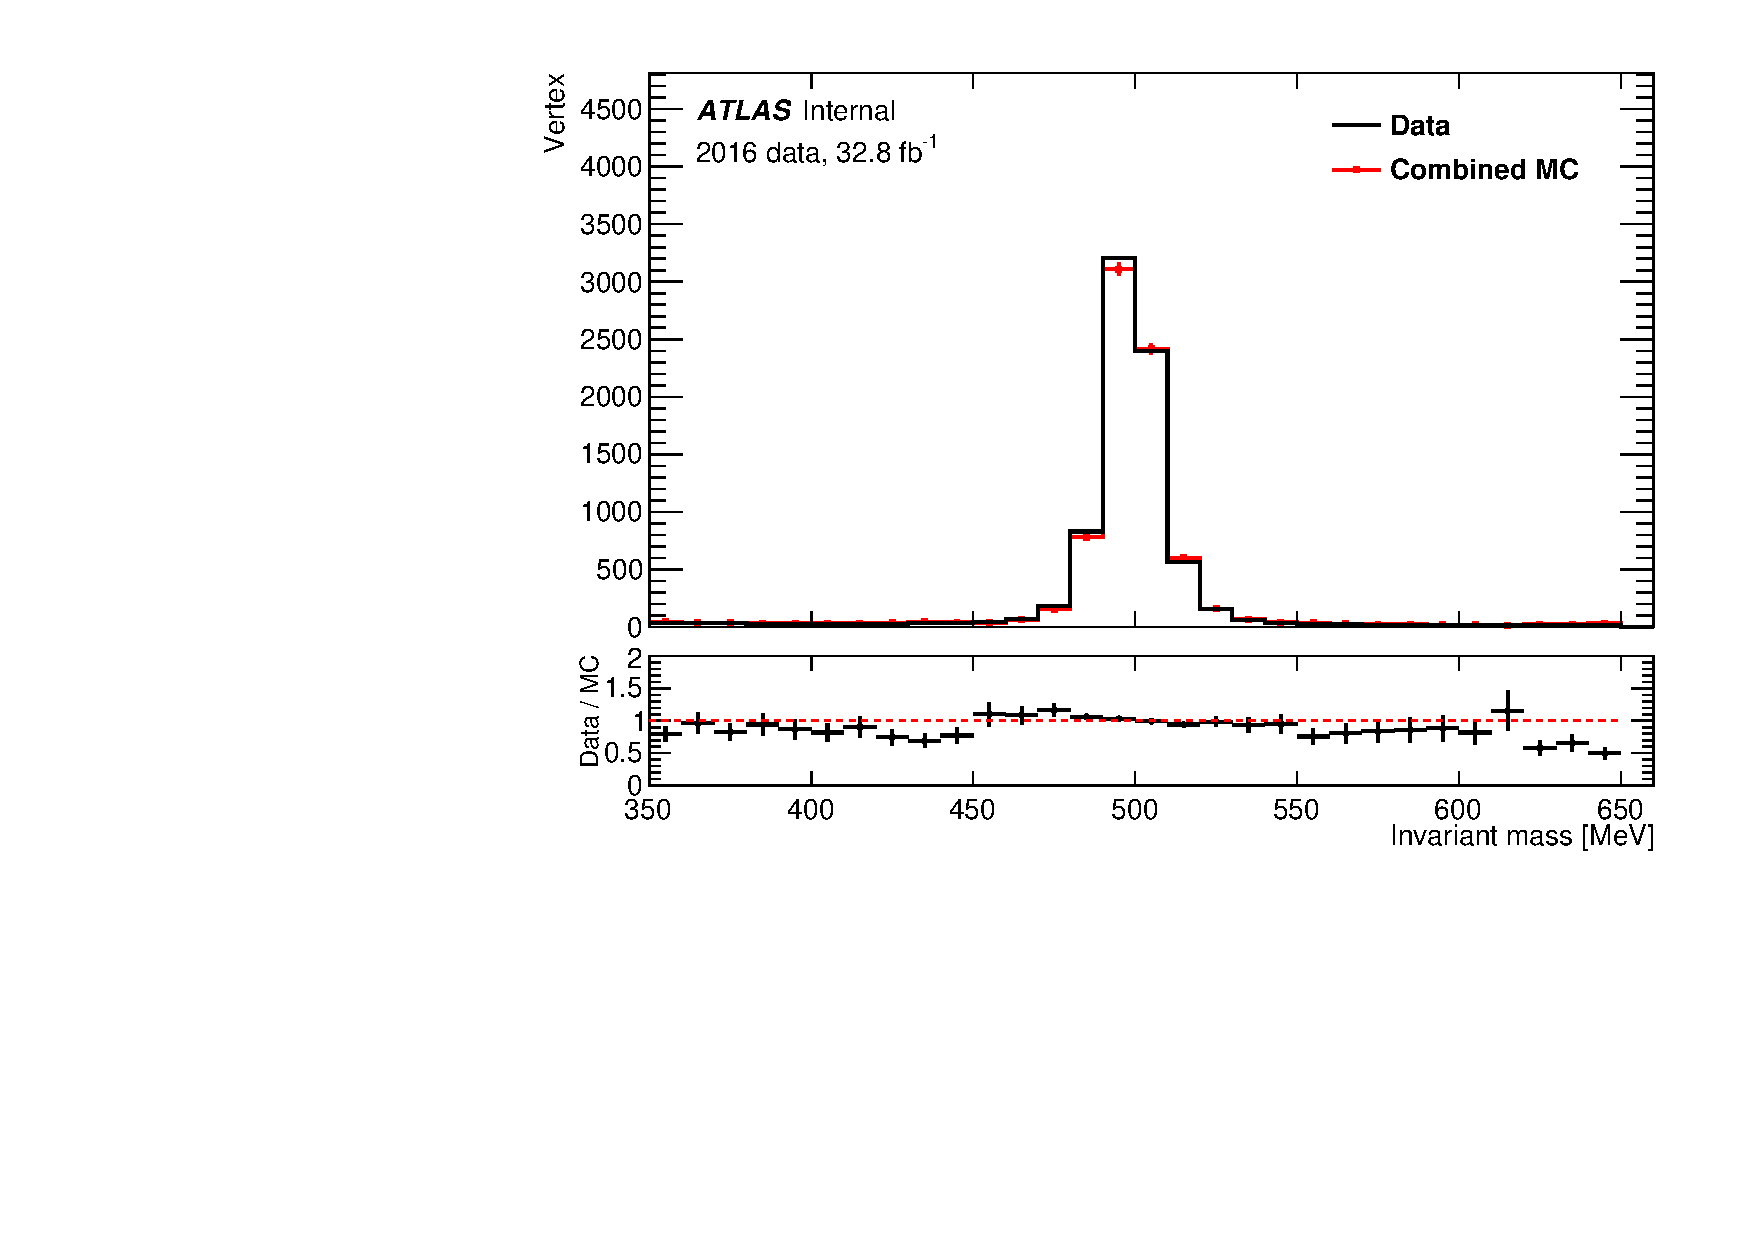
\includegraphics[width=0.45\textwidth]{figures/m_syst_Ks_M.pdf}}
    \subfloat[]{\label{subfig:Ks_pt}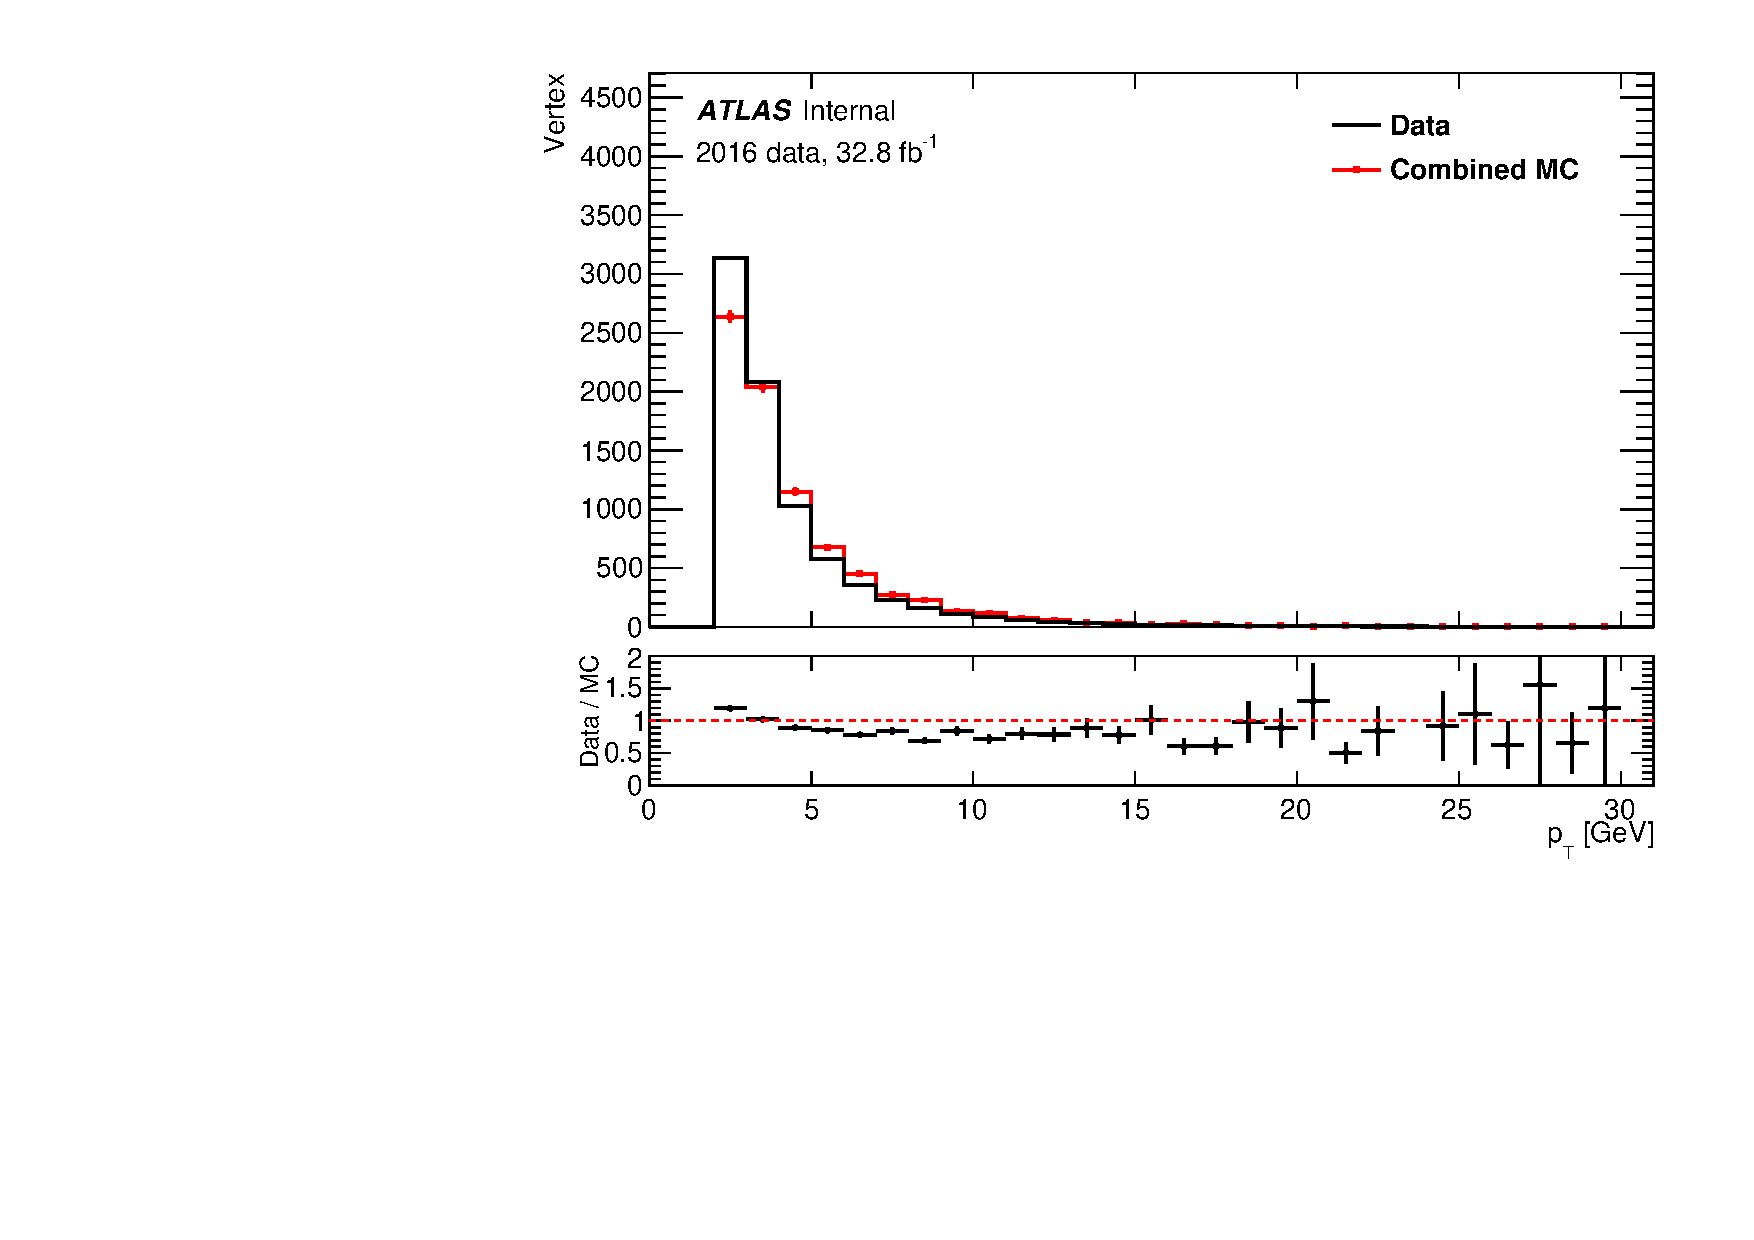
\includegraphics[width=0.45\textwidth]{figures/m_syst_Ks_pt.pdf}} \\
    \subfloat[]{\label{subfig:Ks_mu}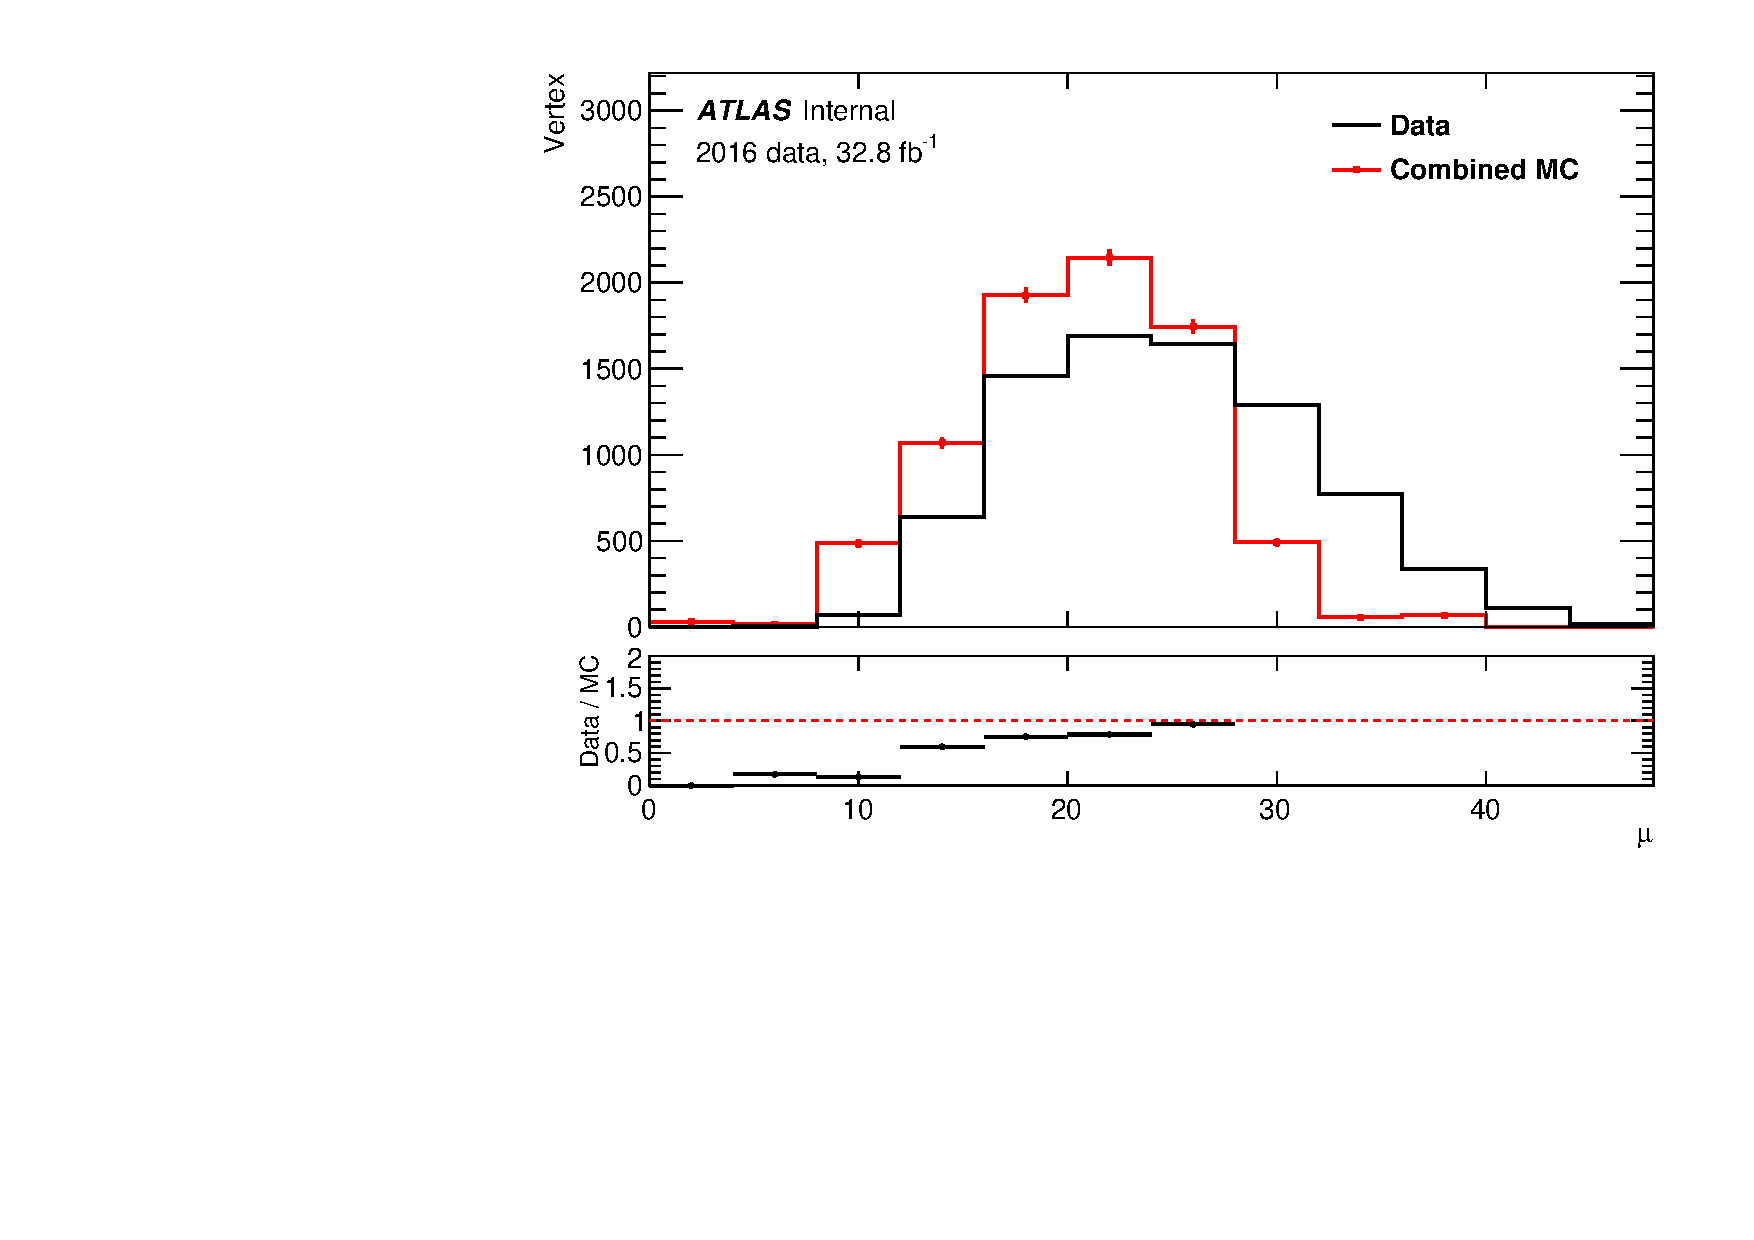
\includegraphics[width=0.45\textwidth]{figures/m_syst_Ks_mu.pdf}}
    \subfloat[]{\label{subfig:Ks_r}\includegraphics[width=0.45\textwidth]{figures/m_syst_Ks_r.pdf}}  \\
    \subfloat[]{\label{subfig:Ks_z}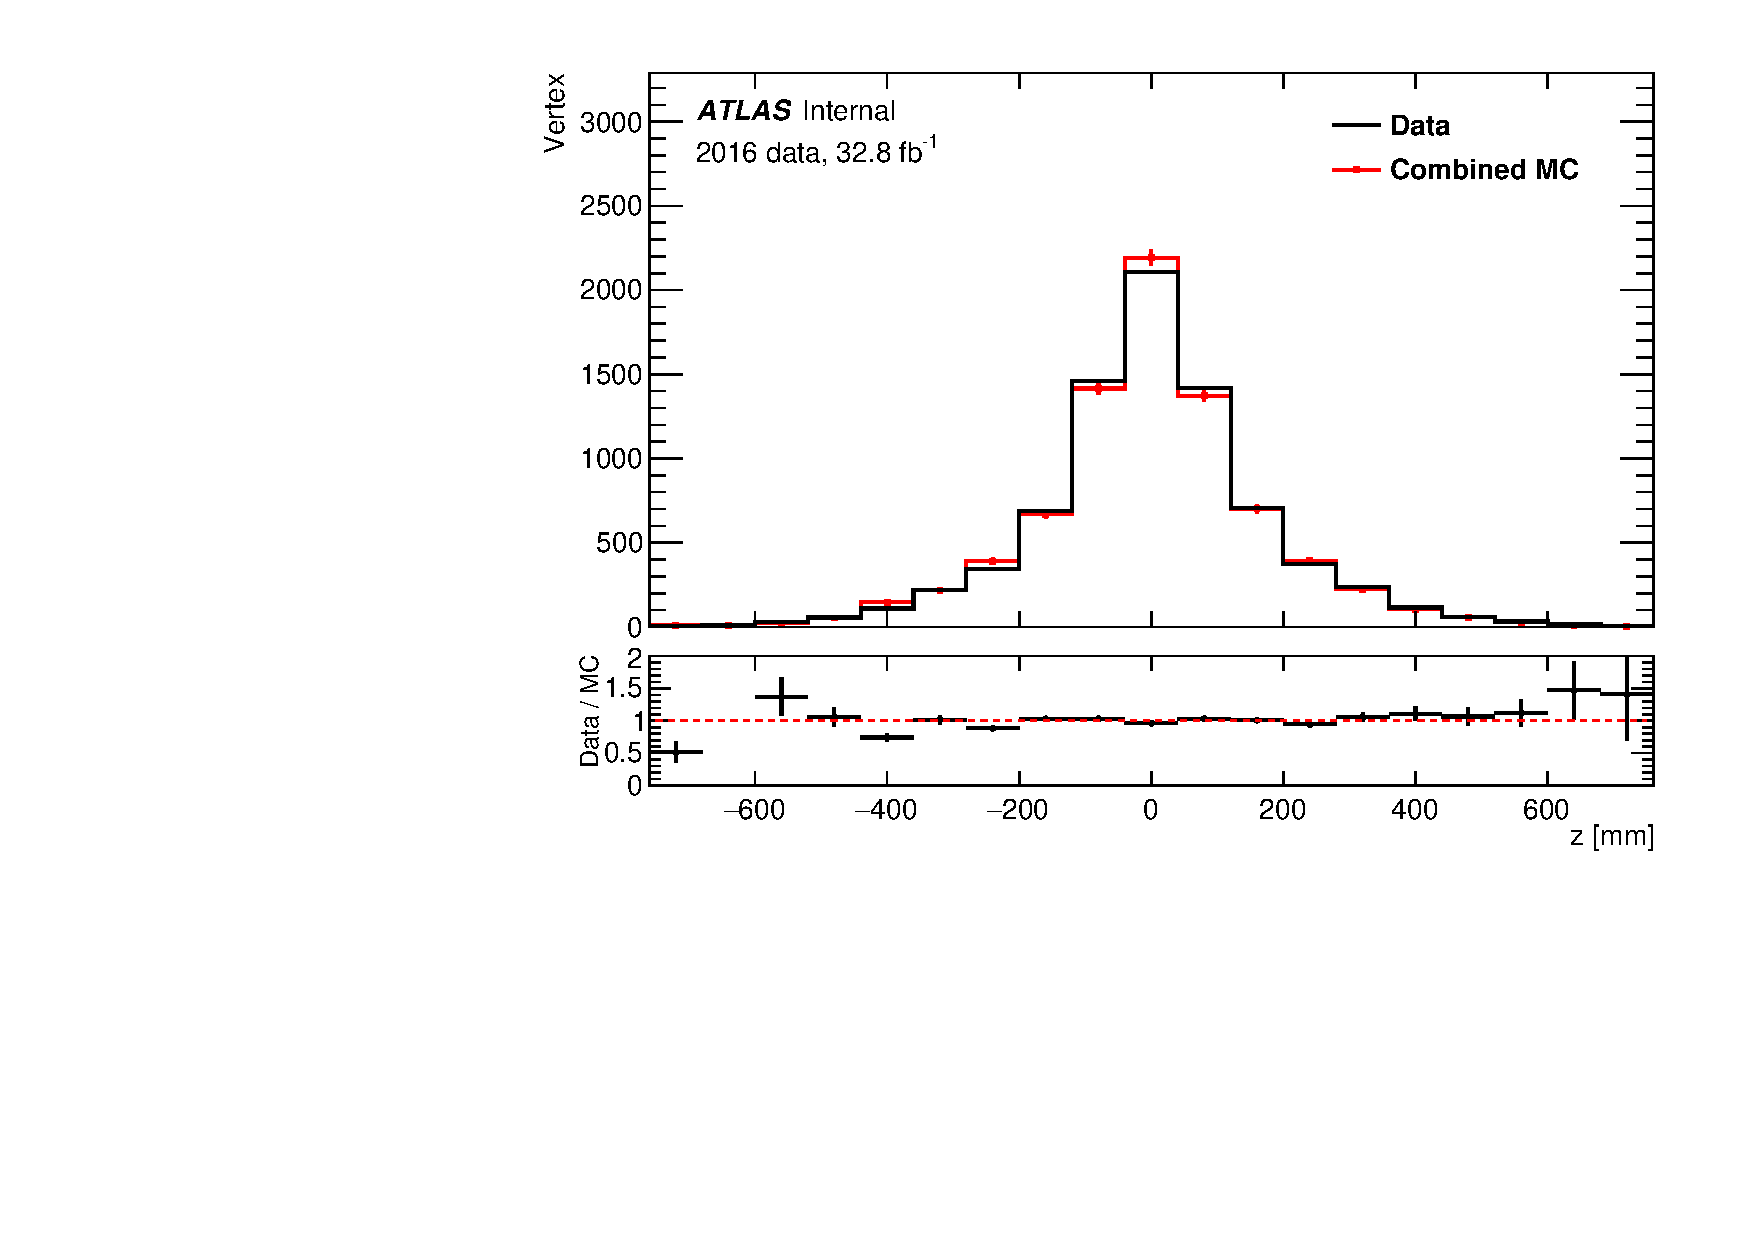
\includegraphics[width=0.45\textwidth]{figures/m_syst_Ks_z.pdf}} 
    \subfloat[]{\label{subfig:Ks_l}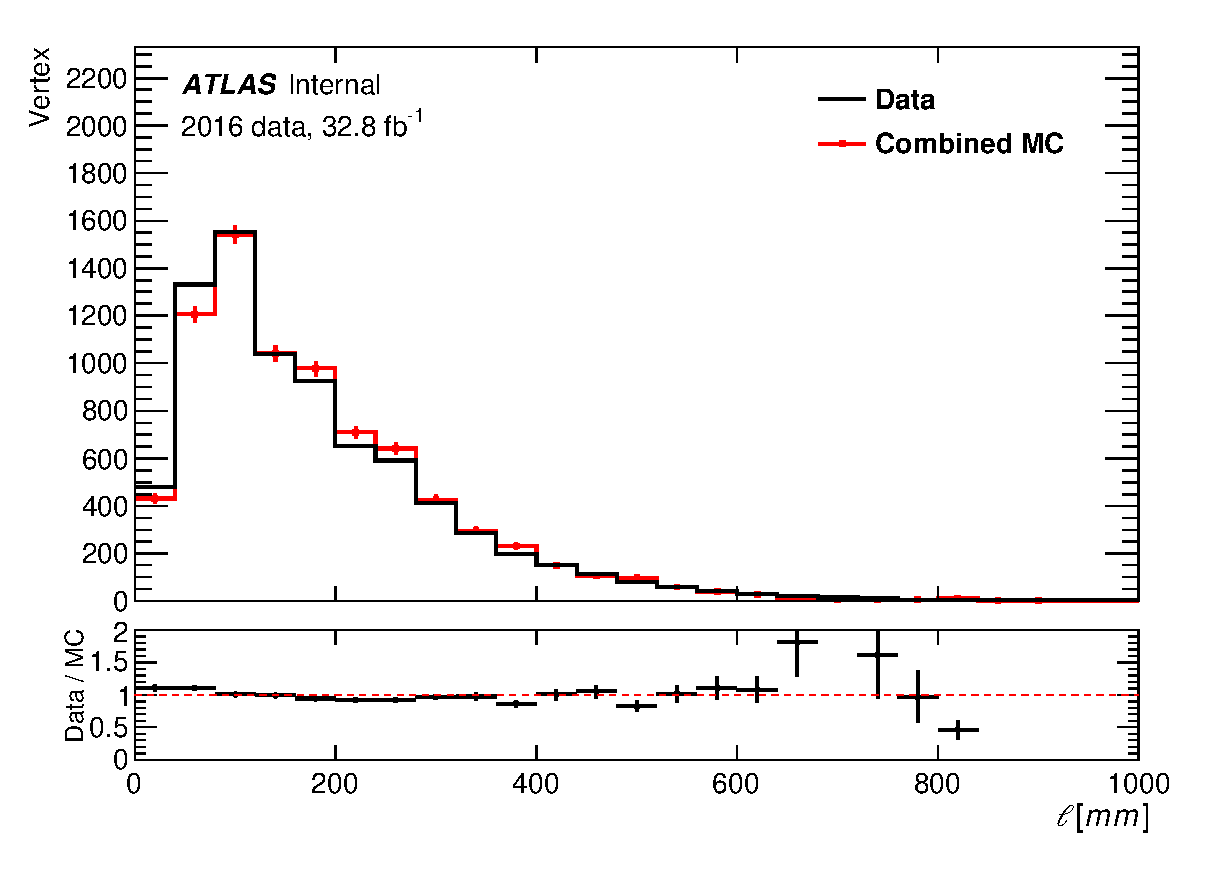
\includegraphics[width=0.45\textwidth]{figures/m_syst_Ks_l.eps}} \\
    \caption{Comparison of the (a) invariant mass, (b) $p_{T}$, (c) $\mu$, (d) transverse, (e) longitudinal position, and (f) decay length of $K_{S}$ in the data with the MC samples. Data is normalized to MC. In (d), the red dashed lines indicate the four Pixel layers and the first layer of SCT. The green dotted lines indicate the Inner Support Tube (45.5 mm) and Pixel Support Tube (229 mm).}
    \label{fig:Ks_data_MC}
\end{figure}

$K_{S}$ vertices found in the data and MC samples are binned in decay radius, $r$, and the $K_{S}$ yields in each bin are estimated from a fit using Breit-wigner. Figure~\ref{fig:Ks_fit} shows a few representative $K_{S}$ mass distributions (others are included in Appendix~\ref{app:syst_Ks_fit}). Background is negligible and hence not included in the fit. The estimated $K_{S}$ yields are normalized to the number of $K_{S}$ found in the lowest $r$ bin since the expected number of $K_{S}$ in the data samples is unknown. 

%\begin{figure}[tb]
\begin{figure}[!htb]
    \centering
    \subfloat[]{\label{subfig:Ks_fit_MC_1}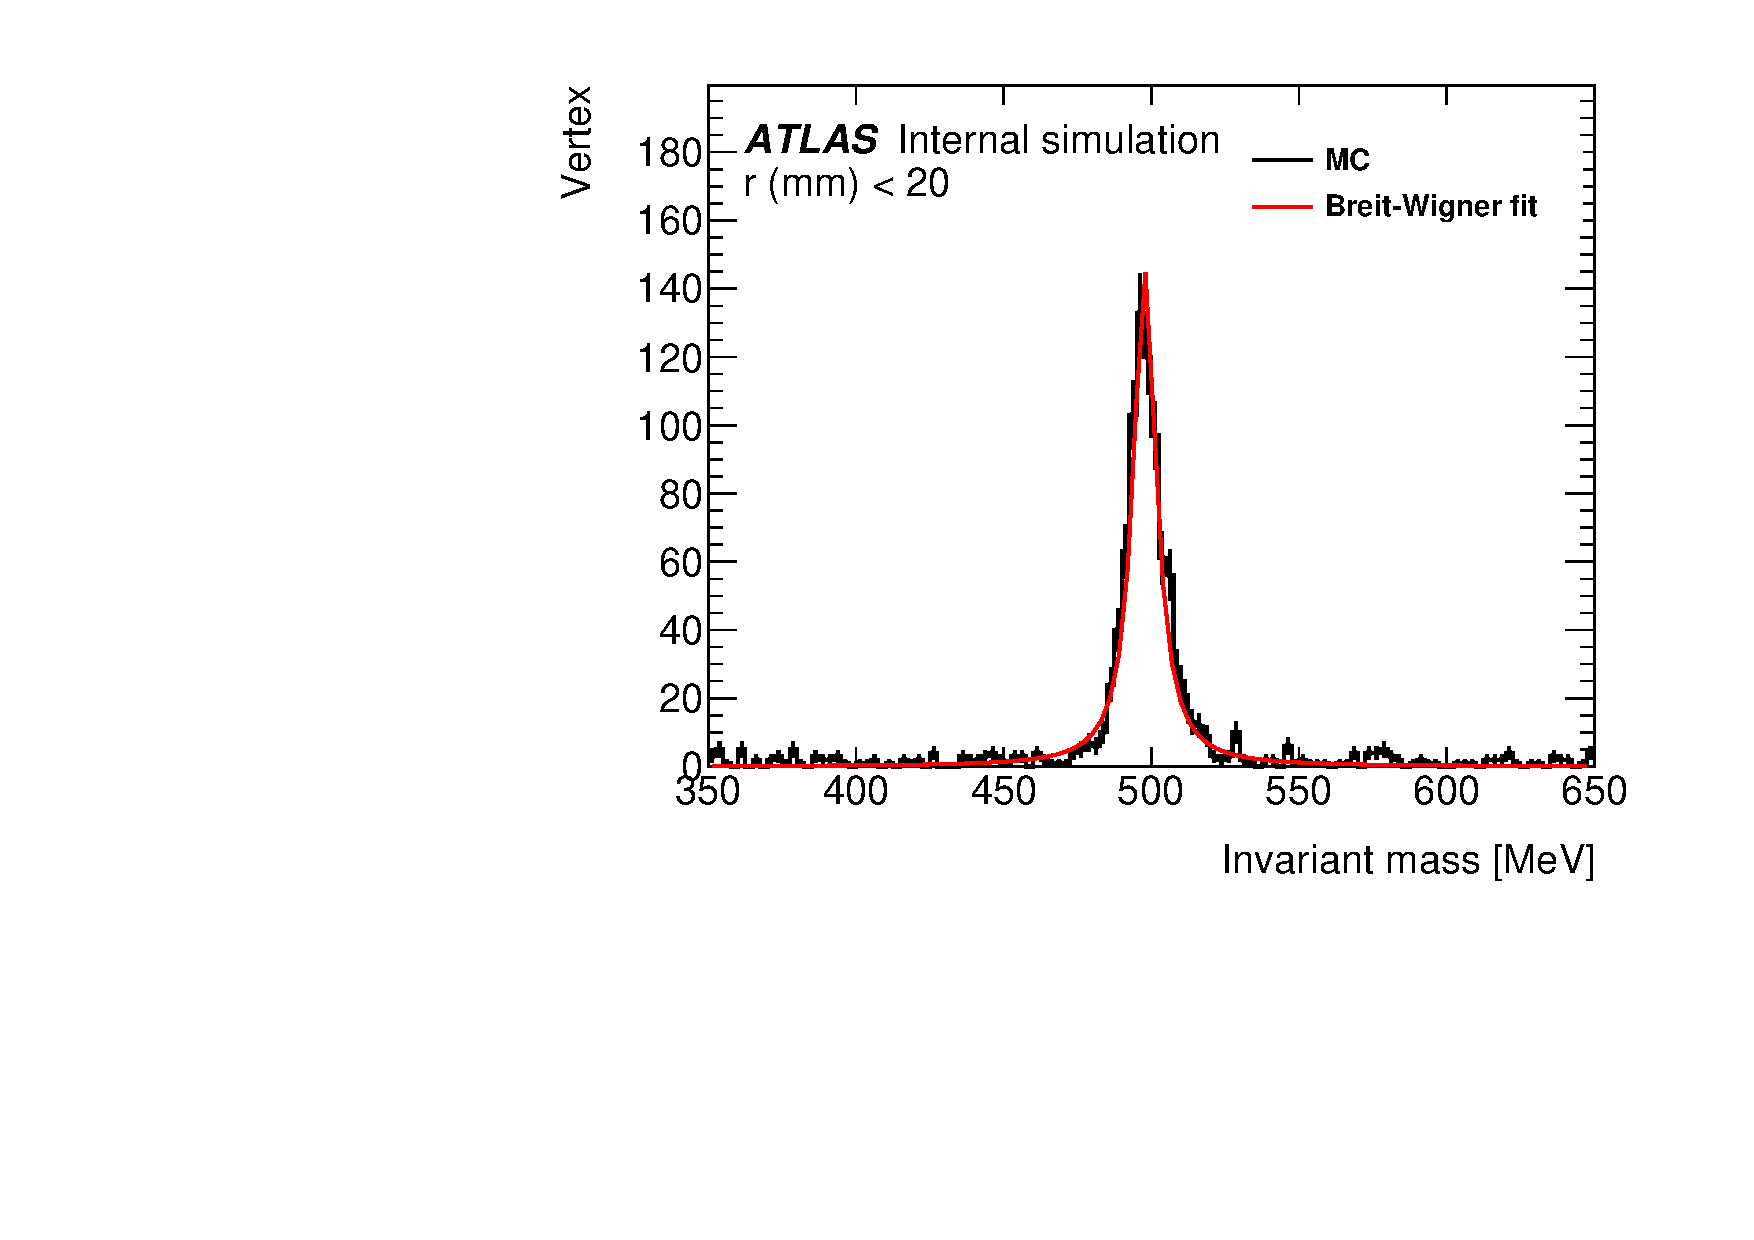
\includegraphics[width=0.45\textwidth]{figures/m_syst_Ks_Combined_MC_1}}
    \subfloat[]{\label{subfig:Ks_fit_MC_2}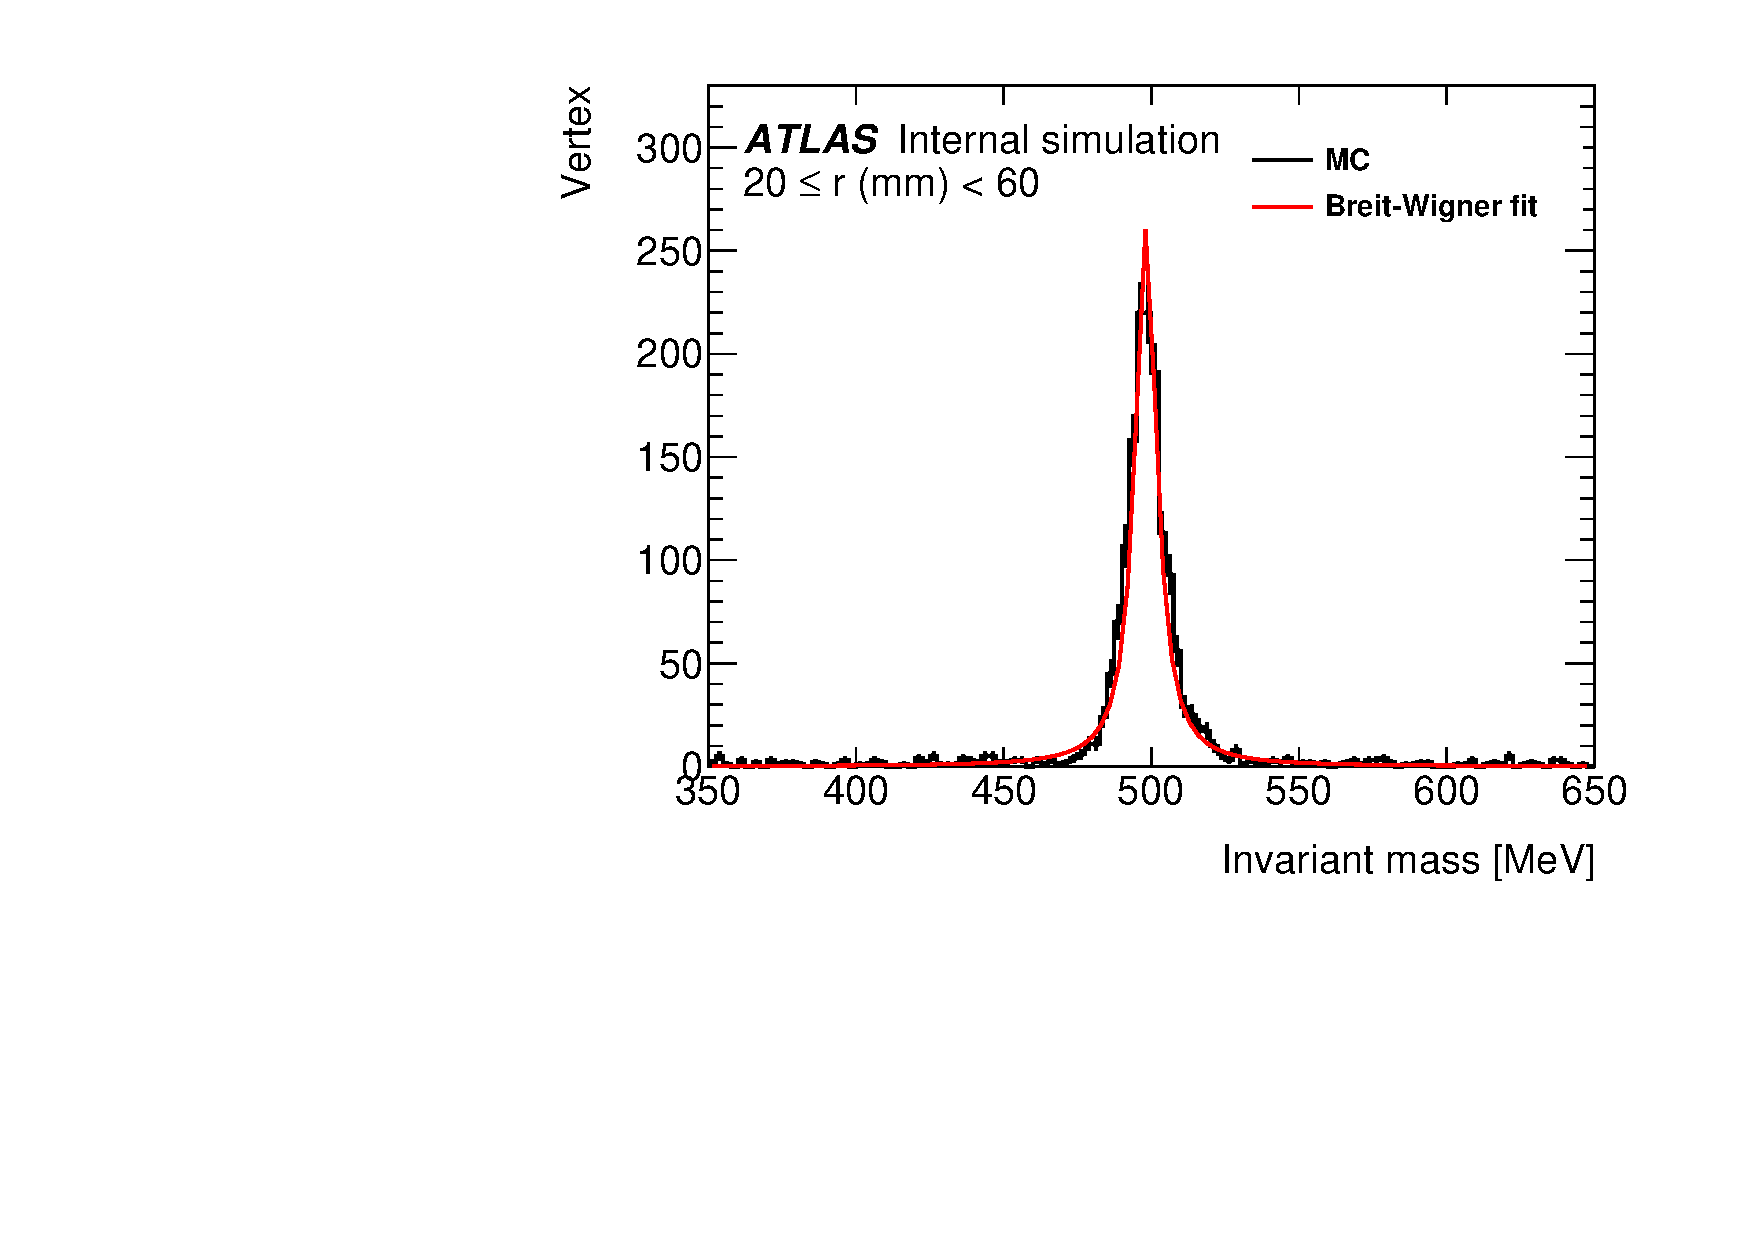
\includegraphics[width=0.45\textwidth]{figures/m_syst_Ks_Combined_MC_2}} \\
    \subfloat[]{\label{subfig:Ks_fit_Data_1}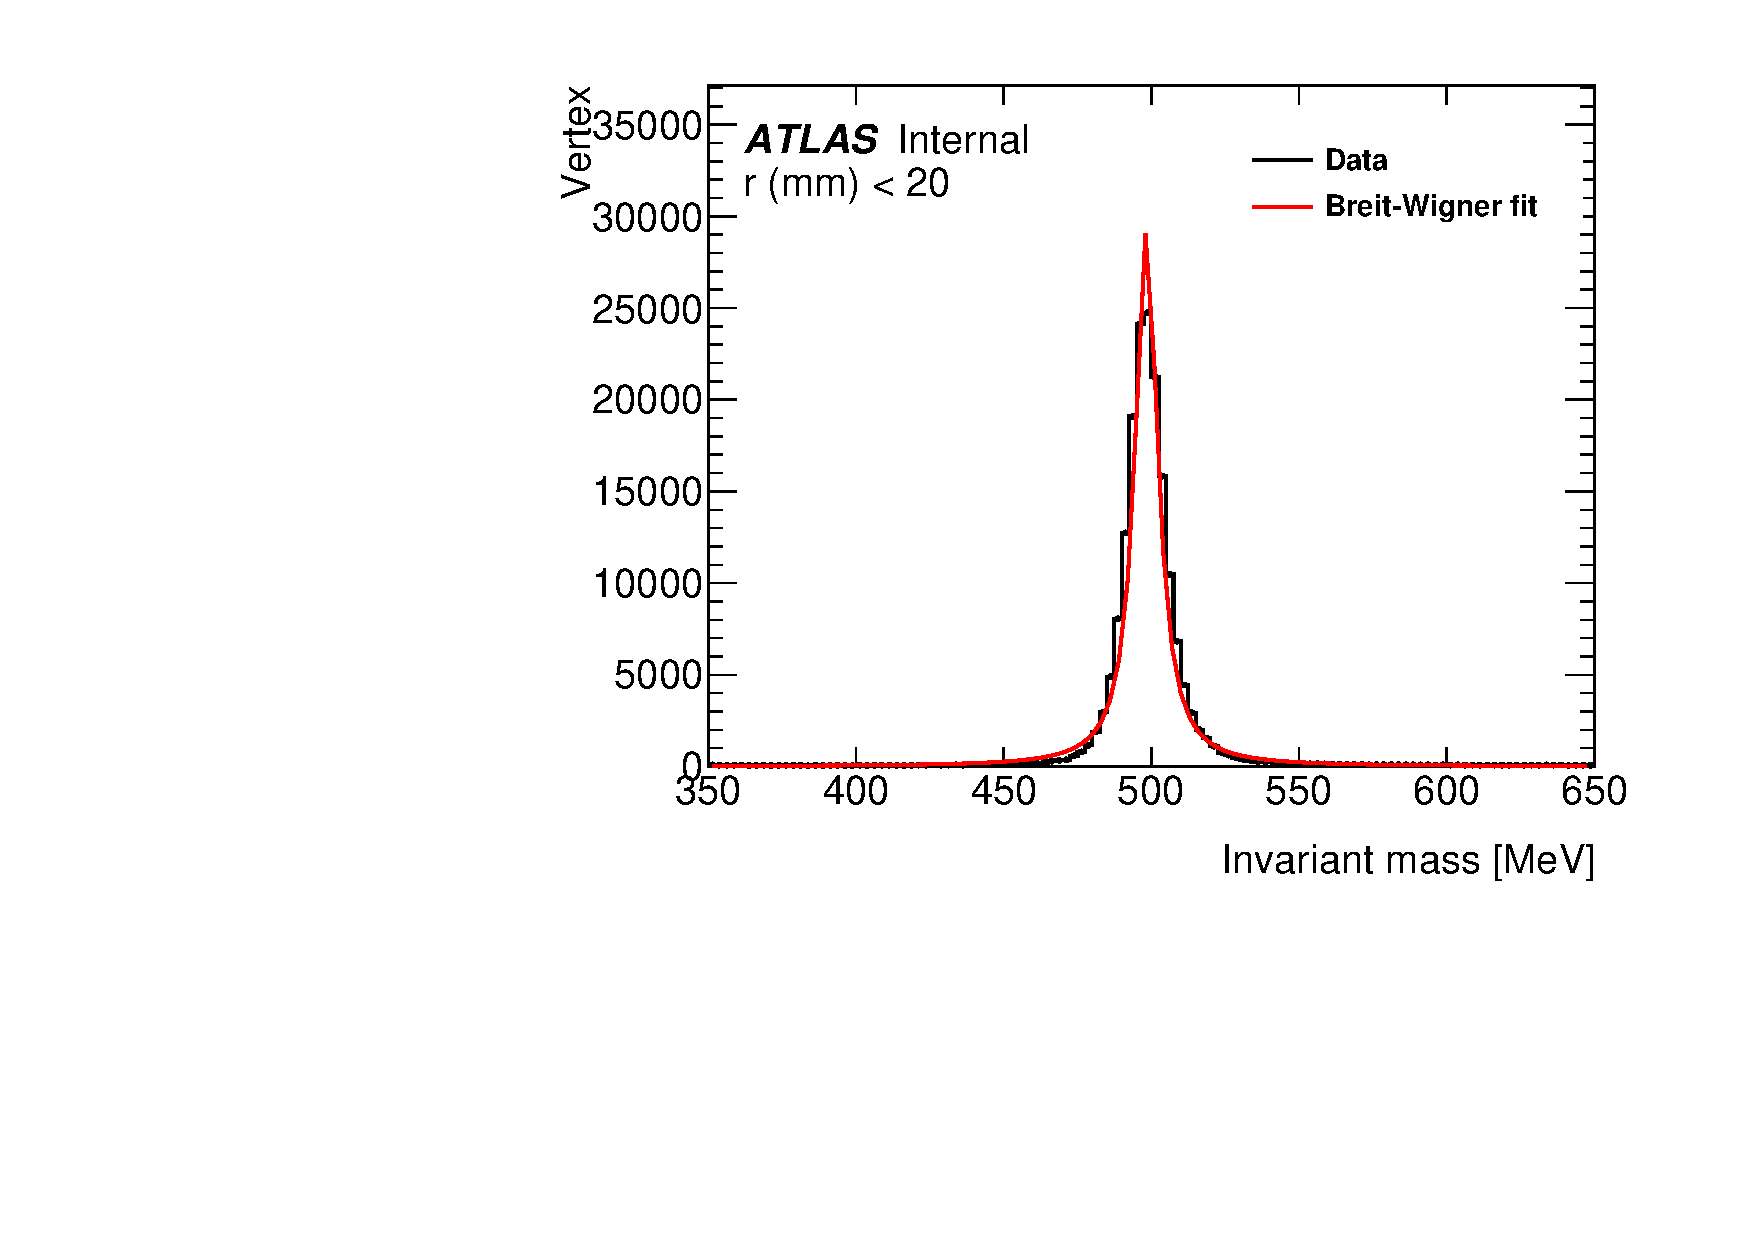
\includegraphics[width=0.45\textwidth]{figures/m_syst_Ks_Data_1}}
    \subfloat[]{\label{subfig:Ks_fit_Data_2}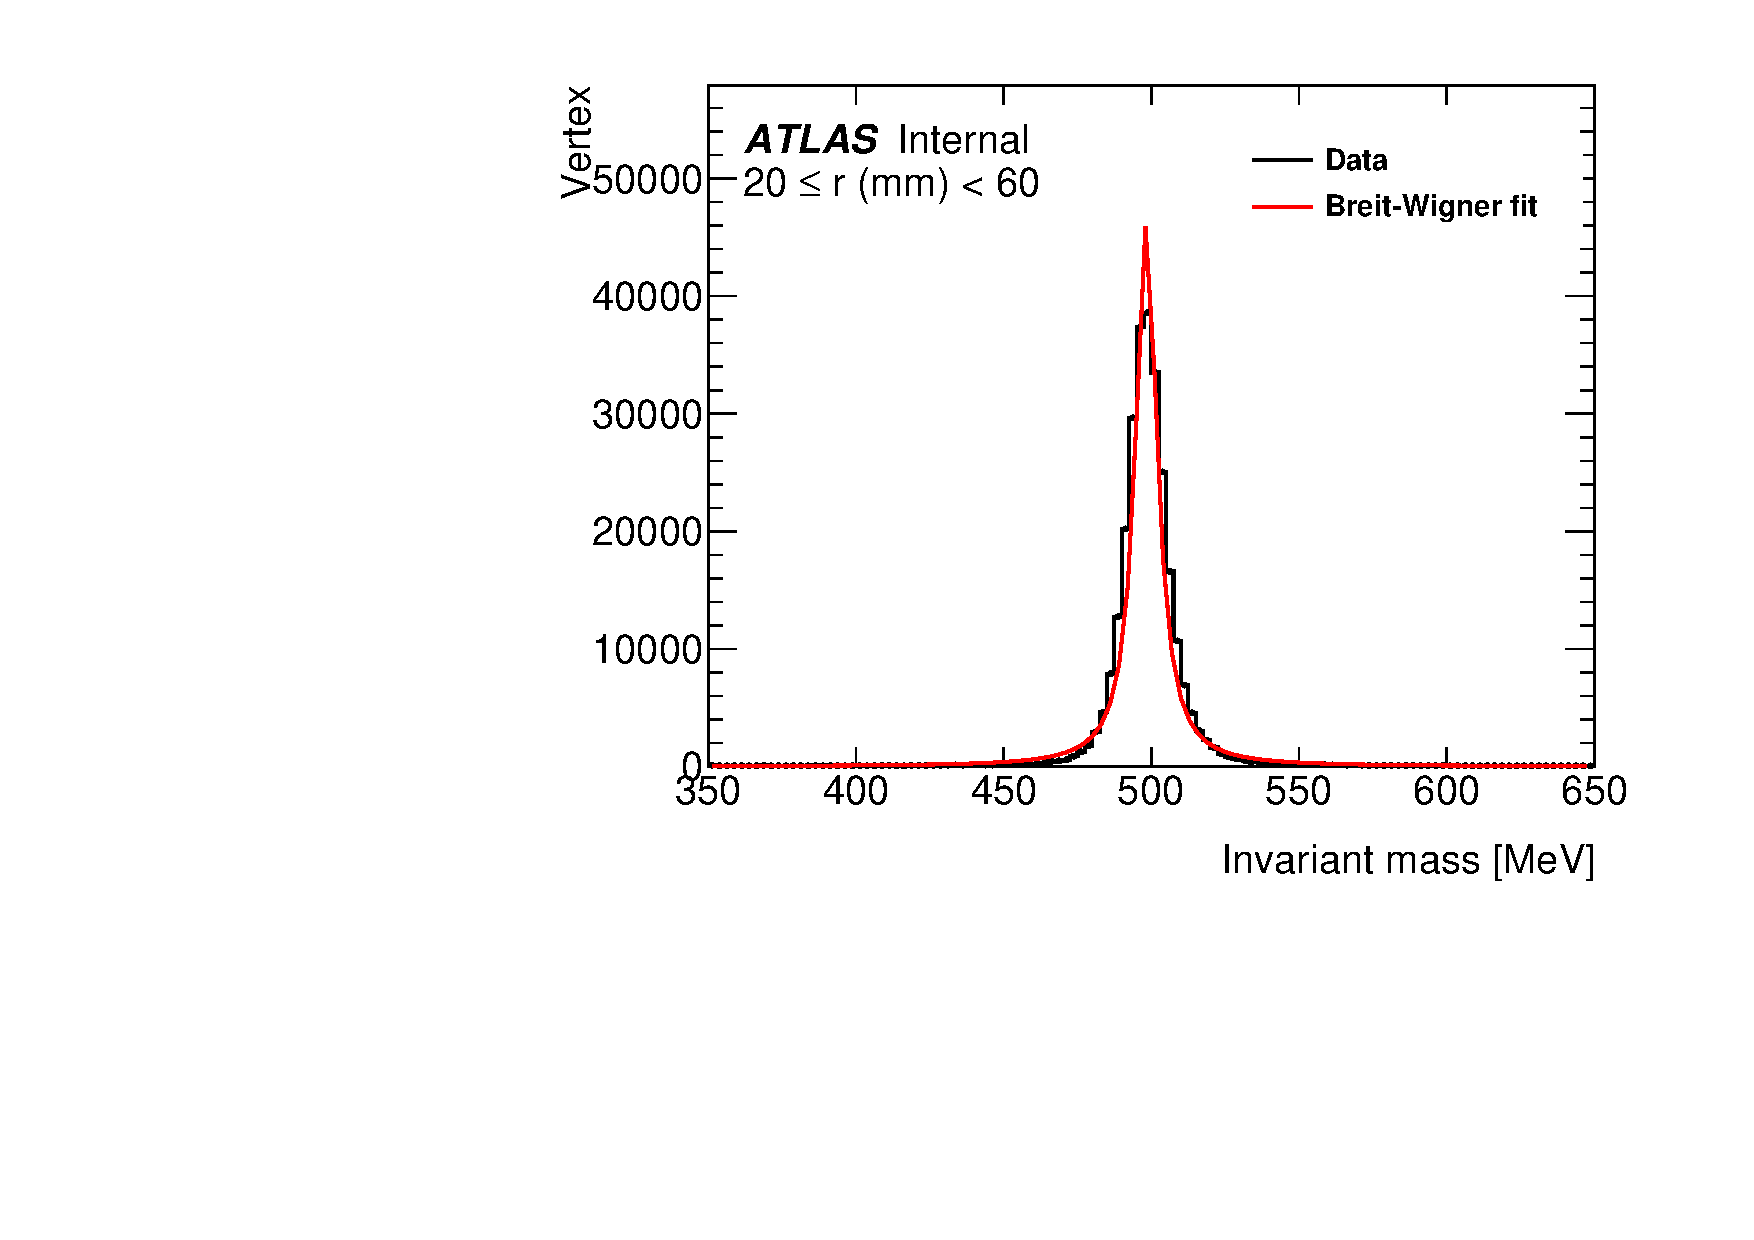
\includegraphics[width=0.45\textwidth]{figures/m_syst_Ks_Data_2}}
    \caption{Representative distributions of the $K_{S}$ invariant mass for (a) $r$ < 20 mm, and (b) 20 $<r<$ 60 mm in the background MC sample. The corresponding plots from the data sample are shown in (c) and (d). The mass distributions are fitted with a Breit-Wigner.}
    \label{fig:Ks_fit}
\end{figure}

%The systematic uncertainty in the lowest bin is taken from the run 2 study \cite{Aad:2011hd}. 
%The ratio of $K_{S}$ vertex yields in each bin of $r$ to $K_{S}$ vertex yields in the lowest $r$ bin is compared between the data and the background MC samples in Figure~\ref{fig:Ks_double_ratio}.
The $K_{S}$ yield, normalized to the yield with $r <$ 20 mm, is compared to the MC in Figure~\ref{fig:Ks_double_ratio}. The lower pane shows the double ratio,

\begin{equation}
\frac{N^{\mathrm{data}}_{R}}{N^{\mathrm{data}}_{R_{0}}} \bigg/ \frac{N^{\mathrm{MC}}_{R}}{N^{\mathrm{MC}}_{R_{0}}}
\label{eq:ks_double_ratio}
\end{equation}

which shows deviation from unity with increase of $r$. The difference in yield is then convoluted with the $r$ distribution of $Z'$ to estimate the systematic uncertainty in tracking and vertexing.

\begin{figure}[!htb]
	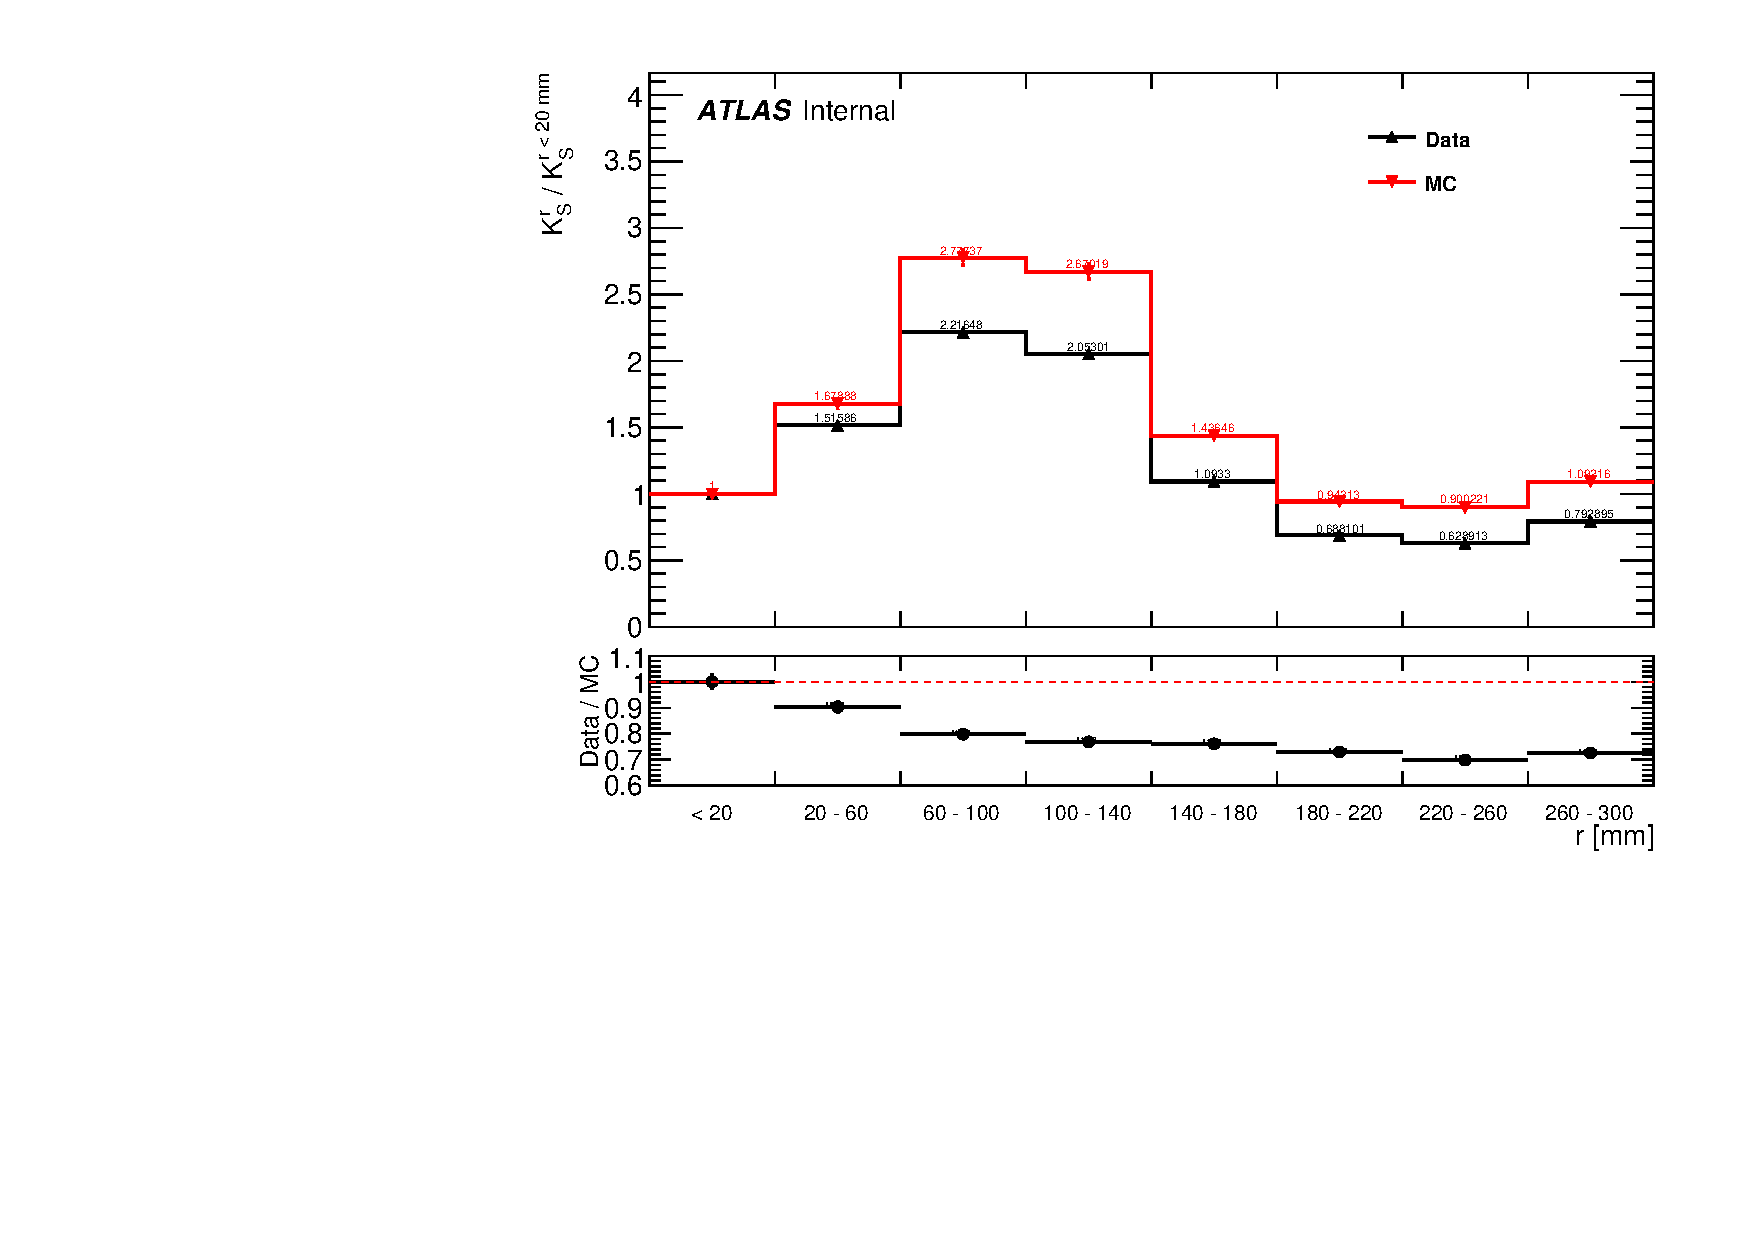
\includegraphics[width=0.50\textwidth]{figures/m_syst_Ks_ratio.pdf}
	\centering
	\caption{The radial distribution of $K_{S}$ yield, normalized to the lowest $r$ bin in the data and MC samples. The lower pane shows the double ratio as defined in the text.}
	\label{fig:Ks_double_ratio}
\end{figure}



\subsection{Systematic uncertainties on lepton identification}
\label{sec:syst_leptonID}

\subsection{Systematic uncertainties on trigger efficiency}
\label{sec:syst_trigger}
